\documentclass[a4paper]{article}

\usepackage[T1]{fontenc}
\usepackage[adobe-utopia]{mathdesign}
\usepackage[protrusion=true,expansion=true]{microtype}
\usepackage{xcolor}
\usepackage{natbib}
\usepackage{graphicx}
\usepackage[utf8]{inputenc}

\definecolor{darkblue}{rgb}{0,0,0.5}

\usepackage[colorlinks=true,
        urlcolor=darkblue,
        anchorcolor=darkblue,
        linkcolor=darkblue,
        citecolor=darkblue,
        pdfauthor={Georg Jung},
        pdfkeywords={educational tools, pseudo-code, virtual machine,
          parser, interpreter},
        pdftitle={Psudo-code virtual machine},
        pdfsubject={Bachelor second interim report for the faculty for MET,
          the German University in Cairo GUC
          (http://met.guc.edu.eg/)}]{hyperref}
\usepackage{url}

\author{Tarek Fouda}
\title{Pseudo-code virtual machine. Second Interim report}

\begin{document}

\maketitle
\section{Introduction}
Pseudo code Algorithum is a code that is taught for student who are new to computer science and coding.
It simply allows them to understand how to assign variables, execute (while,for,do) loops, and how to check for a condition to execute the "if" or the "else" part.
A lot of these new students face a lot of problems in understading the meaning of Pseudo Code, what does the code exactly do and how the variables are assigned and so on. Tracing such a code isn't easy for such students, and they do not know where the code went wrong except from the feed back of the instructor through grading the tests, quizes or the assignments. It's really hard for them to understand the mechanism of Pseudo code algorithm from just a paper, as they can not see any execution happens, they are not aware of how the variables are assigned, neither they are aware of how the loop is executed and how a while loop -for example- stops when the condition is false. Their understanding to such an algorithum needed something more enhanced to teach them the mechanism of such an algorithm.

\subsection{Pseudo-code interpreter approach}
From this point the idea of creating a tool that helps such students literally understand what goes on inside the code, and how it's executed line by line. This interpreter simply is the mirror of the code written by the student, it highlights the errors existing in the code, shows what variables are assigned and the new values assigned to them and finally it translates what happens in the code through a graphical user Interface.
This tool simply allows the student to freely write his/her code and by pressing a compile button all the errors are highlighted. Also by compiling the code an arrow should appear on the very first line, this arrow goes down when the student wants to, after every line is finished, the variables assigned, the loops executed and the conditions checked should appear in a different window and here is the magic of this tool, as it translates exactly the smallest details that happen in the code.

\newpage

\section{How to start on this tool?}
\subsection{The programming language}
To start on how to implement such an interpreter with the above functions, I thought of implementing the tool either in Java or in Haskell. Haskell is a functional programming language and it is more easier to write a lot of grammars and rules in Haskell, but on the other hand, I'm used more to implementing in Java, besides this tool requires a Graphical User Interface GUI which can not be done using Haskell, so It was decided to code and implement this tool using Java programming language.

\subsection{Java parser generator (Antlr)}

Our mind was made up with the language used in implementing in this tool, choosing the specific and efficient Java parser generator was left to begin with the tool. There are many of Java parser generators like (Antlr, JavaCC, BYACC/J.. etc).

The two most popular Java parser generators were Antlr and JavaCC. I had to research and compare between them in terms of differences, flexibility and learning curve.

I started to search more for Antlr and JavaCC, Antlr home page provided me with more convenient documentation and explanation about how the generator and the lexer work.
On the other hand JavaCC homepage was a bit difficult for me to understand the documentation out of it.
Another advantage of Antlr was that it produces parser source code in various languages but on the other hand, JavaCC only produces java. By more researches I found out that Antlr was more developer-friendly than JavaCC.
Moreover Antlr had Eclipse plugins and that was an advantage as the project uses Graphical User Interface and the most easiest way to integrate all the code together with the GUI is through eclipse, so Antlr having an Eclipse IDE was a huge advantage for me.

\subsection{How to start with Antlr}
Installing Antlr is pretty easy after following the instruction presented in the home page of Antlr website www.antlr.org .
\newpage
Installing Antlr for UNIX and WINDOWS are shown, but in my case I was using windows, installing Antlr for windows was as shown in Figure 1.
$$ $$
\begin{figure}[ht]
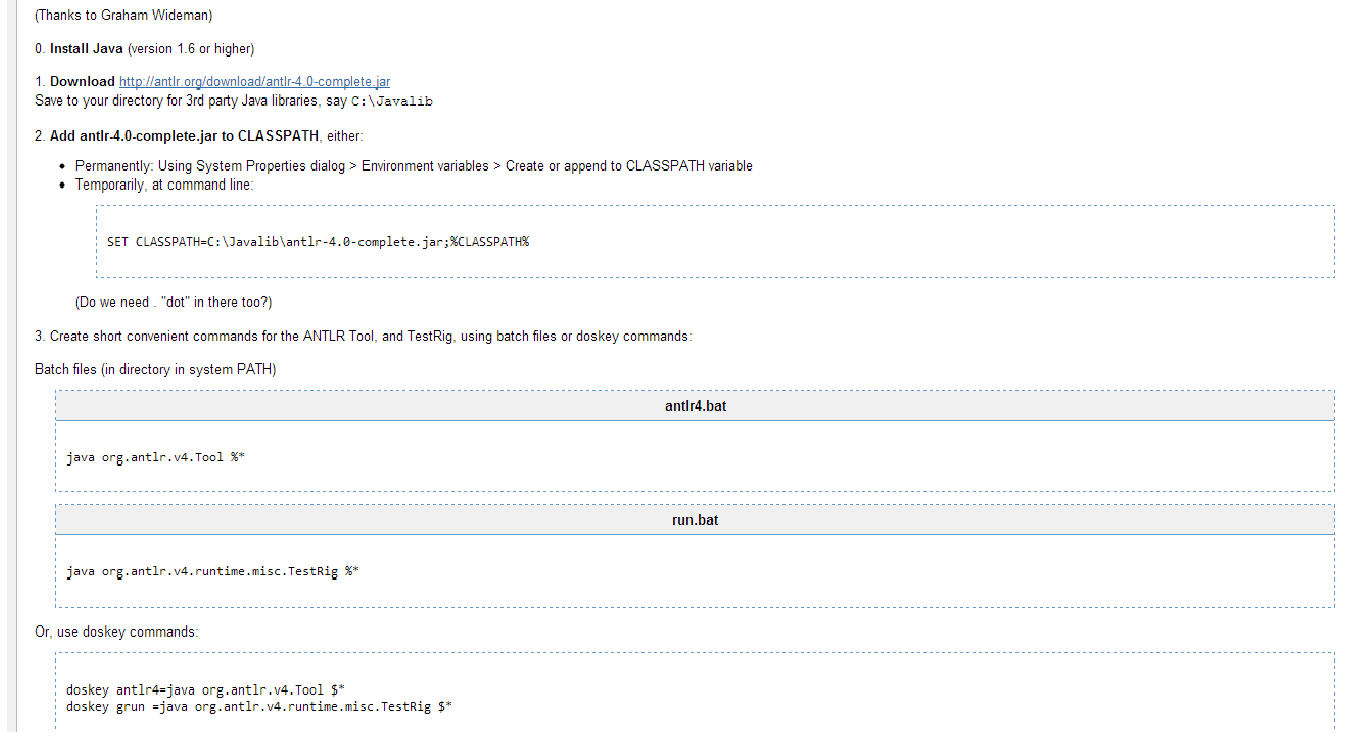
\includegraphics[width = \paperwidth]{1.png} 
\caption{ANTLR installation for windows users}
\end{figure}

$$ $$
\newpage

After successefully installing Antlr on your machine you need to test your installation by typing the following two commands in your terminal in Figure 2. 

$$ $$
\begin{figure}[ht]
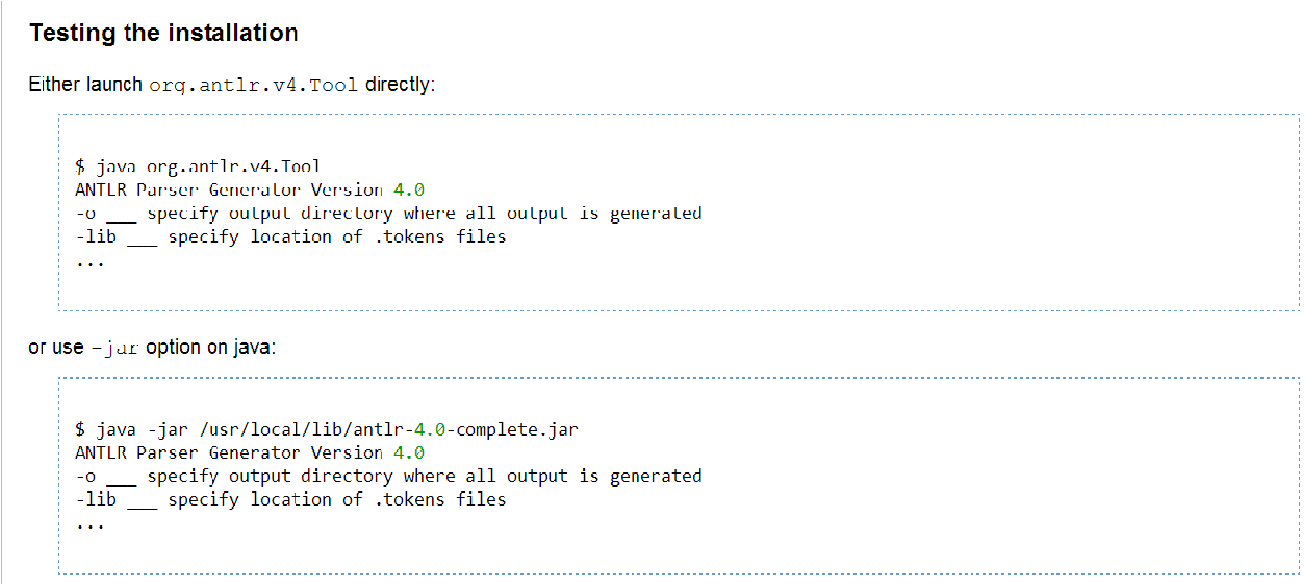
\includegraphics[width =\paperwidth]{2.png} 
\caption{Testing ANTLR installation}
\end{figure}
$$ $$
\newpage
In the rest of the tutorial there is a simple grammar to teach you how to write a grammar using Antlr the grammar is simply consister of a start rule $r$ and two other Lexer rules which are the identification and White spaces ( $ID$ , $WS$). Also there is the -gui that produces the parse tree of a grammar as shown in Figure 4.
$$ $$
\begin{figure}[ht]
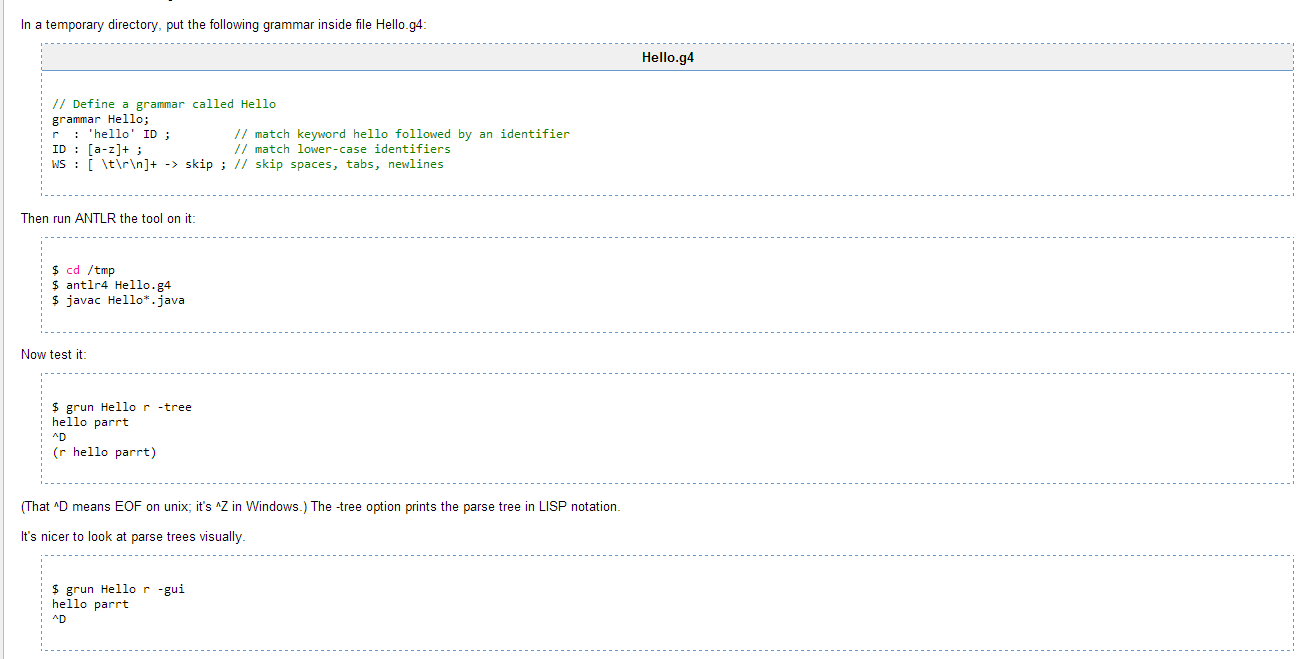
\includegraphics[width = \paperwidth]{3.png} 
\caption{}
\end{figure}
\newline 
\begin{figure}[ht]
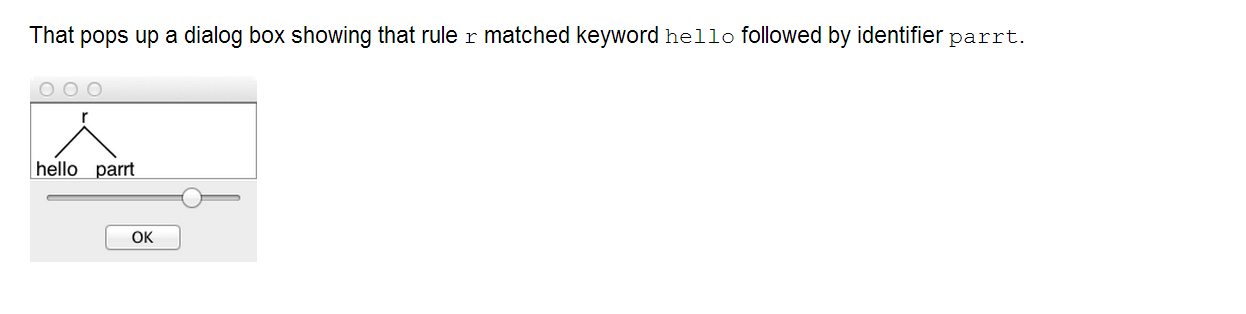
\includegraphics[width = \paperwidth]{4.png} 
\caption{}
\end{figure}
$$ $$
Now Antlr is installed on the machine and waiting for a grammar $.g$ file to be written. One of the reasons we chose Antlr over JavaCC is that Antlr has eclipse plugins and IDE, we've searched for how to install this plugin on eclipse to enhance our developing infrastructure.

Thanks to Scott Stanchfield who introduced a tutorial on how to install Antlr 3.x IDE on eclipse.
$ http://vimeo.com/8015802 $.  
.
By following this tutorial we now have Antlr installed on eclipse and ready to be in use.
Starting a new Antlr project will create a $.g$ file where the grammar should be written in. Regarding our tool we have a grammar that covers all the combinations and tokens any Pseudo code would have.
\subsection{GRAMMAR}
The grammar was as the following:
$$ $$
<ALGORITHM>      ::= $'algorithm' $ <ID> [$ 'inputs$ <DECLIST>]? \newline \centerline{
[$'outputs'$ <DECLIST>]?} \newline \centerline {[$'localvar'$ <DECLIST>]? $'begin'$ <STATEMENT> $'end'$ }

$$ $$

<INDEX>   ::= $'['$ <ARITHEXPR> $']'$

$$ $$

<INDEXING>::= $'['$ <VALUE> $'...'$ <VALUE> $']'$

$$ $$ 

<IDLIST> ::=  <ID> $','$ <IDLIST> | <ID>
$$ $$ 

<ASSIGN>  ::= $'set'$ <ID> $'to'$ <ID>

$$ $$

<ASSIGNLIST> ::= <ASSIGN> $','$ <ASSIGNLIST> | <ASSIGN>

$$ $$

<DECL> ::= $'number'$ <ID> [<INDEXING>]? | $ 'data' $ <ID> \newline  \centerline {[<INDEXING>]?}
\newpage
$$ $$

<DECLLIST> ::= <DECL> $','$ <DECLLIST> | <DECL>

$$ $$
<STATEMENT> := \centerline{  <ASSIGNMENT>} \newline \centerline {| <SEQUENTIAL>} \newline \centerline{ |  <CONDITIONAL> } \newline \centerline{ |  <ITERATIVE>} \newline \centerline{  | <PRINT> } \newline \centerline { | <READ>} \newline \centerline {| <INVOCATION>}


$$ $$

<ASSIGNMENT> ::= $'set'$ <ID> [<INDEX>]? $'to'$ (<ARITHEXPR> | \newline \centerline{ <DATAEXPR>)}

$$ $$

<SEQUENTIAl> ::= <STATEMENT> $';'$ <STATEMENT>

$$ $$

<CONDITIONAL> ::= $'if'$ <CONDITION> $'then'$<STATEMENT> $'else'$ \newline \centerline {<STATEMENT>} \newline \centerline
{$'endif'$} \newline \centerline {
| $'if'$ <CONDITION> $'then'$ <STATEMENT> $'endif'$}

$$ $$

<ITERATIVE>  ::= $'while'$ <CONDITION> $'do'$ <STATEMENT> $'loop'$

$$ $$

<PRINT> ::= $'print'$ (<DATAEXPR> | <ARITHEXPR>)

$$ $$

<READ> ::= $'read'$ <IDLIST>

$$ $$
<INVOCATION> ::= $'run'$ <ID> [$'inputs'$ <ASSIGNLIST>]? \newline \centerline {[$'outputs'$<ASSIGNLIST>]? $'done'$}

$$ $$

\newpage

$$ $$
<CONDITION> ::= <DISJUNCTION>

$$ $$
 <DISJUNCTION> ::= <CONJUNCTION> $'or'$ <DISJUNCTION> \newline \centerline {|  <CONJUNCTION>}
 
 $$ $$ 
 <CONJUNCTION> ::= <NEGATION> $'and'$ <CONJUNCTION> \newline \centerline { | 
 <NEGATION>}
 
 $$ $$
 <NEGATION> ::= $'not'$ <ATOM> | <ATOM>
 
 $$ $$
 
 <ATOM>::= <BOOLEXPR> | $'('$ <DIJUNCTION> $')'$

$$ $$
<BOOLEXPR> ::= <ARITHEXPR> ($'='$ |  $'<>'$ | $'<'$ | $'>'$ | $'<='$ | $'>='$ ) <ARITHEXPR>

$$ $$ 
<ARITHEXPR> ::= <MULTIPLICATION> ( $'+'$  | $'-'$ ) <ARITHEXPR> \newline \centerline{ | <MULTIPLICATION>}

$$ $$

<MULTIPLICATION> ::= <NEGEXP> ($'*'$  |$'/'$ ) <MULTIPLICATION> \newline \centerline{ | <NEGEXP> }
$$ $$
<NEGEXP> ::= $'-'$ <VALUE> | <VALUE> |$'('$ <ARITHEXPR>$')'$

$$  $$

<VALUE> ::= <ID> [<INDEX>]? | <INTEGER>

$$ $$
 <INTEGER> ::= ($'1'$..$'9'$)($'0'$..$'9'$)* 
 
 $$ $$ 
<ID> ::= ($'a'$..$'z'$ | $'A'$..$'Z'$)+ 

\newpage

\subsection{Antlr and Eclipse IDE}

Now we have a grammar and an ANTLR plugin on eclipse, There are three views of the grammar ( Grammar, Interpreter, RailRoad view) 

\subsubsection{Grammar view}
The grammar view simply displays the grammar you have written with highlighting the lines that contain error.
A simple grammar view is in the following figure.
\newline
\begin{figure}[ht]
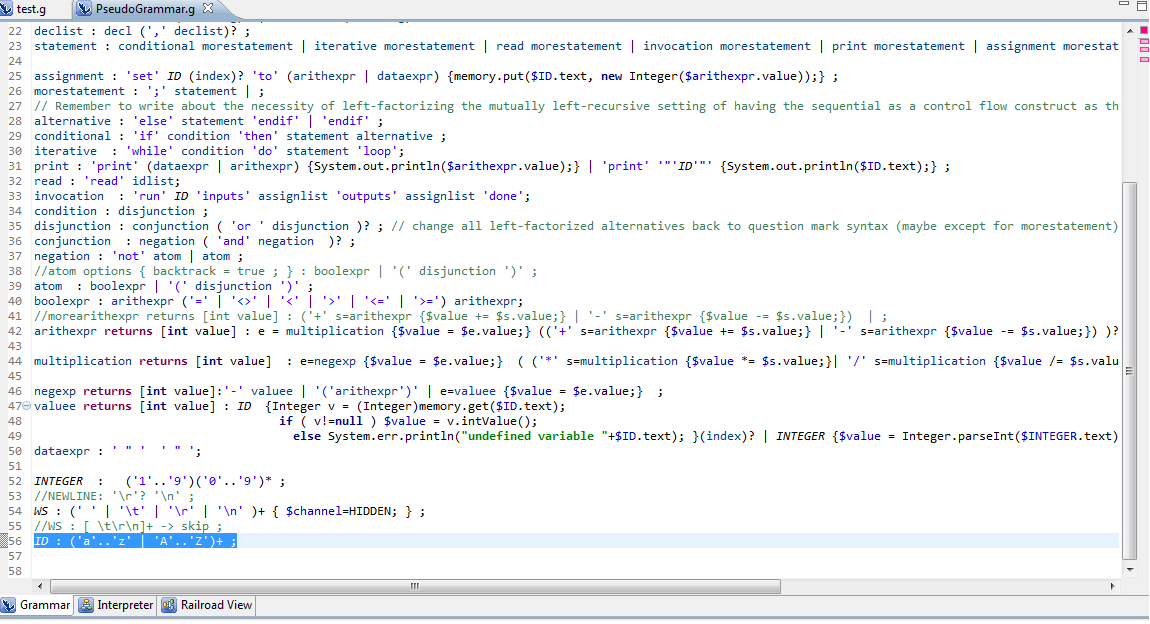
\includegraphics[width = \paperwidth]{5.png} 
\caption{Grammar View.}
\end{figure}
\newline

\subsubsection{Interpreter view}
The Interpreter view is simply consisted of two main things, the first thing is a Text Field where the developer could write a sample code or a mini code to test whether everything is write or not. The second thing is a Displaying windows that shows the output of the entered code mentioned above. In other words, The developer types a sample code in the text field as shown in the below figure and the Interpreter produces the Parse Tree of this code as shown below.
\newline
\begin{figure}[ht]
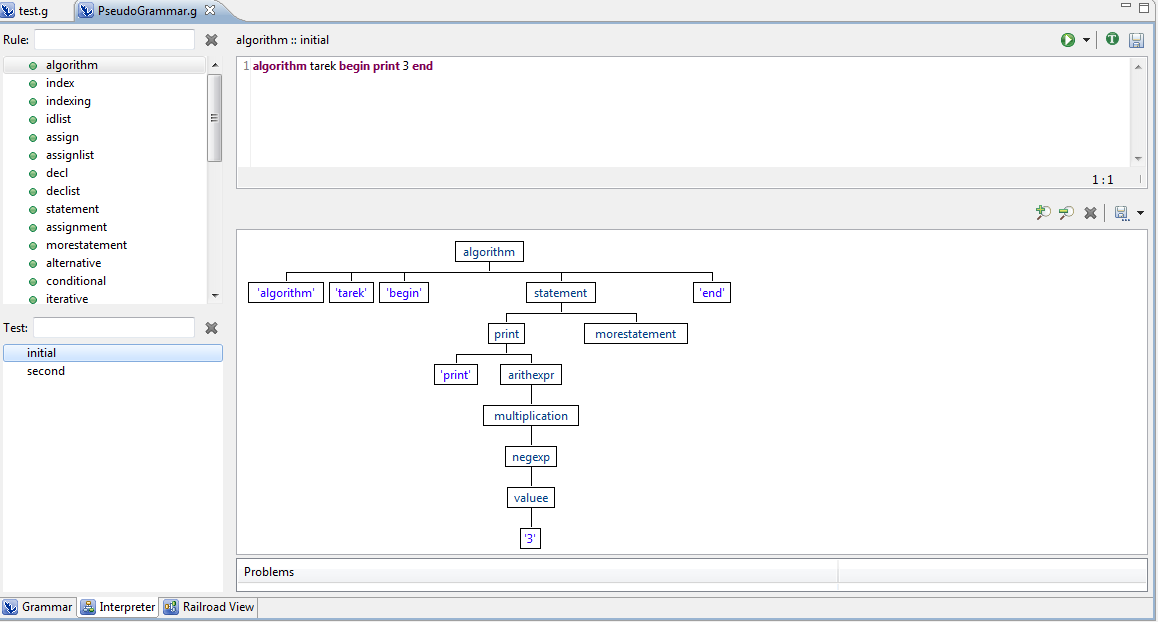
\includegraphics[width = \paperwidth]{6.png} 
\caption{Interpreter View}
\end{figure}
\newline
\subsubsection{Rail Road view}

The Rail Road view is a view which the developer could check what every rule in the grammar do and require. for example $algorithm$ rule mentioned in this section, This rule needs $'algorithm'$ and an $ID$. The $'inputs'$ and the $'outputs'$ are not required to be there, they are optional. The Rail Road view shows that all. Check the below figure to understand the task of this view more precisely and accurately.
\newline
\begin{figure}[ht]
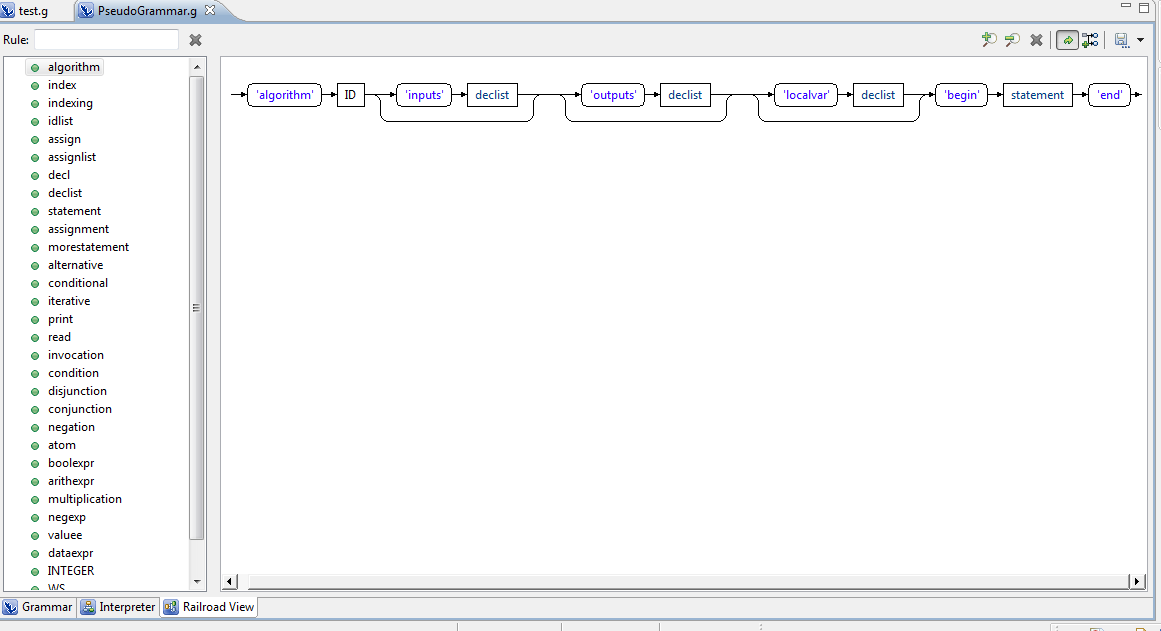
\includegraphics[width = \paperwidth]{7.png} 
\caption{Rail Road View.}
\end{figure}


\section{Left Factorizing the mutually left recursive tokens}

 \begin{quotation}
 Writing grammars, one will encounter left-recursive rules. As ANTLR is a recursive-descent parser, it cannot cope with them and thus they have to be removed. But what is a left-recursive rule exactly? It is a recursive rule which calls itself on the left-edge of a global alternative. An example would be:
$$ $$ 
$a   :    a b
    |    b
    ;$
    
    $$ $$
ANTLRworks can resolve this problem and turns rule a into
$$ $$
$a   :    b+;$

$$ $$
But ANTLRworks can do this automatically only for the above kind of left-recursive rules, which exhibit the left recursion within the implementation of the recursive rule itself. I would call these single left-recursive (SLR) rules. The other kind are mutually left-recursive (MLR) rules where the left-recursion occurs over several rule invocations. The simplest example would be the following:
$$ $$
$a   :    b
    |    c
    ;$
 $$ $$ 
 $$ $$
$b   :    a
    |    c
    ;$
    $$ $$
Rule a references rule b, while rule b references rules a. A more complex example would show such a 're-reference' taking place after many subsequent rule invocations. As stated above, the resolvement has to be done manually here.
 \end{quotation}
 
 That was said by $ Johannes Luber$ on May 2, 2008. He was declaring on www.antlr.org website that ANTLR 3.x can not resolve the problem of the left recursive rules. On the other hand, ANTLR 4 was capable of resolving such a problem but unfortunately there was no ANTLR 4 plugin on eclipse, only ANTLR 3.x existed. That was the reason the above grammar mentioned in the previous section needed modification and left factorizing to eliminate the left-recursive problem existed in the grammar.
 \newpage
 Simply left factorizing the rules was kind of an easy task for lots of rules, for example,  rules like :
 
 $$ $$
 $$ $$
 <DISJUNCTION> ::= <CONJUNCTION> $'or'$ <DISJUNCTION> \newline \centerline {|  <CONJUNCTION>}
 
 $$ $$ 
 <CONJUNCTION> ::= <NEGATION> $'and'$ <CONJUNCTION> \newline \centerline { | 
 <NEGATION>}
 
 $$ $$
 $$ $$
 
 Eclipse highlighted these two rules as they were left-recursive so this problem was to be resolved manually by gathering the common things in the rule and put it in a temporary rule as follows:
 
 $$ $$
 <MORECONJUNCTION> ::= $'and'$ <CONJUNCTION> | Epsilon
  $$ $$
  <CONJUNCTION> ::= <NEGATION> <MORECONJUNCTION>
 $$ $$
 
 and the same goes for $DISJUNCTION$ rule:
 
 $$  $$
 <MOREDISJUNCTION> ::= $'or'$ <DISJUNCTION> | Epsilon
 $$ $$
 <DISJUNCTION> ::= <CONJUNCTION> <MOREDISJUNCTION>
 $$ $$
 
 By this we eliminated the problem of left-recursive but this was not the efficient solution, because an additional rule for all the rules having left-recursive problem was not the optimal solution. Instead these two rules were modified to be as following:
 
   $$ $$
  <CONJUNCTION> ::= <NEGATION> [$'and'$ <CONJUNCTION>]? 
 $$ $$
  <DISJUNCTION> ::= <CONJUNCTION> [$'or'$ <DISJUNCTION>]?
 $$ $$
 
 \newpage
 
 Also an obvious problem appeared in $SEQUENTIAL$ rule as this rule references $STATEMENT$ rule and referenced by $STATEMENT$ rule as well.
 
 $$ $$
<STATEMENT> := \centerline{  <ASSIGNMENT>} \newline \centerline {| <SEQUENTIAL>} \newline \centerline{ |  <CONDITIONAL> } \newline \centerline{ |  <ITERATIVE>} \newline \centerline{  | <PRINT> } \newline \centerline { | <READ>} \newline \centerline {| <INVOCATION>}



$$ $$

<SEQUENTIAl> ::= <STATEMENT> $';'$ <STATEMENT>

$$ $$

A solution was proposed to get over such a problem and that was to eliminate $$SEQUENTIAL$$ rule and replace it by another rule that does not reference $$STATEMENT$$. The following was the solution of such a problem:
 $$ $$
<STATEMENT> := \centerline{  <ASSIGNMENT> <MORESTATEMENT>}  \newline \centerline{ |  <CONDITIONAL><MORESTATEMENT> } \newline \centerline{ |  <ITERATIVE><MORESTATEMENT>} \newline \centerline{  | <PRINT> <MORESTATEMENT> } \newline \centerline { | <READ><MORESTATEMENT>} \newline \centerline {| <INVOCATION><MORESTATEMENT>}



$$ $$

<MORESTATEMENT> ::=  $';'$ <STATEMENT> |

$$ $$

Grammar is now not left-recursive and contain no errors

\end{document}

%%% Local Variables: 
%%% mode: latex
%%% TeX-master: t
%%% End: 